\documentclass[a4paper, 12pt, addpoints]{exam}
\usepackage{IfbaListas}
%==============================================================
\NumList{3 - Recuperar} %NÚMERO DA LISTA
\Assunto{Lógica}
%==============================================================
%=========================================================
%------------Cabeçalho e rodapé 
%=========================================================
\pagestyle{headandfoot}%{head}%empty
\firstpageheader{}{}{}
\runningheader{\disciplina}{}{Lista \numlist: \assunto}
\runningheadrule
% \copyright \professor
\firstpagefooter{}{}{Pag. \thepage\ de \numpages}
%\iflastpage{Outros templates em \href{http://gg.gg/profwaldexsantos}{gg.gg/profwaldexsantos}
\runningfooter{}{}{Pag. \thepage\ de \numpages}
\runningfootrule
%===============================================================
%INFORMAÇÕES SOBRE A AVALIAÇÃO
\nomeInst{Instituto Federal da Piauí}
\logoInst{
\includegraphics[scale=0.17]{Figs/IFPIPicosVertical.png}}
\Campus{Picos} %PARA ENSINO FUNDAMENTAL OU MÉDIO-COMENTE ESTA LINHA COM %
\nomeCurso{Análise e Desenvolvimento de Sistemas} %Se não for curso superior, basta comentar esta linha ou deixar em branco
\nomeDisciplina{Matemática Computacional}
\Semestre{1}
\nomeProfessor{Rogerio Figueredo de Sousa}
\Aluno{}
\matriculaAluno{}
%===============================================================
 %CARREGA AS INFORMAÇÕES GERAIS DO PROFESSOR, ESCOLA ETC
%==============================================================

%COMEÇO DO DOCUMENTO
\begin{document}
\info\vspace{-1 cm} %Imprime as informações do cabeçalho programada no pacote 
% inicia a gravacao da resposta no arquivo "ans" cujo nome externo é gabarito 
\Opensolutionfile{ans}[Gabarito]
%*****************************************************************************
\begin{questions}%COMEÇA O AMBIENTE DE QUESTÕES
  \question Seja $\oplus $ o operador ``xor'' (``Exclusive Or'') definido como $P \oplus Q := (P \leftrightarrow Q)'$, onde P, Q, R e S são proposições lógicas quaisquer. Usando a tabela verdade, prove que:
  \begin{enumerate}[a)]
    \item $(P \oplus Q) \Leftrightarrow (P \lor Q) \land (P' \lor Q')$
    \item $P \oplus (Q \oplus R) \Leftrightarrow (P \oplus Q) \oplus R$
    \item $(P \oplus Q) \land (R \oplus S) \Leftrightarrow (P \land R) \oplus (P \land S) \oplus (Q \land R) \oplus (Q \land S)$
    
  \end{enumerate}
  
   \begin{resp}~
    
  \end{resp}

  \question Prove que o operador condicional ($\rightarrow$) é distributivo com todos operadores ($\land, \lor, \rightarrow, \leftrightarrow$). Ou seja, prove os seguintes itens, onde P , Q e R são sentenças lógicas quaisquer:

  \begin{multicols}{2}
    \begin{enumerate}
      \item $(P \rightarrow Q') \lor P'$
      \item $(P \lor (Q \oplus R)) \leftrightarrow ((P \lor Q) \oplus (P \lor R))$
      \item $(P \lor Q') \rightarrow Q'$
      \item $(P \rightarrow (Q \rightarrow R)) \leftrightarrow ((P \rightarrow Q) \rightarrow R)$
      \item $P \leftrightarrow (P' \lor Q')$
      \item $(P \rightarrow (Q \oplus R)) \leftrightarrow ((P \rightarrow Q) \oplus (P \rightarrow R))$
    \end{enumerate}
  \end{multicols}

  \question Considerando as oito sentenças abaixo e assumindo que não há contradição entre elas, descubra o valor lógico (\textbf{V} ou \textbf{F}) de cada sentença. Justifique.
  
    \begin{itemize}
      \item Sentença $\bigtriangleup_1$: Exatamente sete das sentenças desta questão são falsas.
      \item Sentença $\bigtriangleup_2$: Exatamente seis das sentenças desta questão são falsas.
      \item Sentença $\bigtriangleup_3$: Exatamente cinco das sentenças desta questão são falsas.
      \item Sentença $\bigtriangleup_4$: Existem oito sentenças nesta questão.
      \item Sentença $\square_1$: A Sentença $\bigtriangleup_1$ é falsa.
      \item Sentença $\square_2$: A Sentença $\bigtriangleup_2$ é falsa.
      \item Sentença $\square_3$: A Sentença $\square_4$ é verdadeira.
      \item Sentença $\square_4$: A Sentença $\square_4$ é verdadeira.
    \end{itemize}
  

  \begin{resp}~
    
  \end{resp}

  \question  Considerando as quatro sentenças abaixo, a última sentença é verdadeira? Justifique.

  \begin{itemize}
    \item Existem quatro sentenças nesta questão.
    \item Três das sentenças desta questão são falsas.
    \item A última sentença é verdadeira.
    \item Esta lista de exercícios está muito fácil.
  \end{itemize}
  


  \begin{resp}~
  
  \end{resp}

  \question  Usando as regras da lógica proposicional, prove cada argumento abaixo, usando as letras de proposição dadas:
  
  \begin{itemize}
    \item Se o programa é eficiente, executa rapidamente: ou o programa é eficiente ou tem algum bug. No entanto, o programa não executa rapidamente. Logo, ele tem um bug. E, R, B.
    \item Se Jane é a mais popular, ela será eleita. Se Jane é a mais popular, então Carlos vai renunciar. Portanto, se Jane é a mais popular, ela será eleita e Carlos renunciará. J, E, C
    \item Rússia era uma potência superior, e a França não era suficientemente poderosa ou Napoleão fez um erro. Napoleão não fez um erro, mas, se o exército não perdeu, então a França era poderosa. Portanto, o exército perdeu e a Rússia era uma potência superior. R, F, N, A (exército)
    \item Se José tivesse levado as joias ou se a Sra. Krasov tivesse mentido, então um crime teria sido cometido. O Sr. Krasov não estava na cidade. Se um crime tivesse sido cometido, então o Sr. Krasov estaria na cidade. Portanto, José não levou as joias. J, L (mentir), C, T (cidade)
    \item Emília não estava em casa ou, se Patrícia não tivesse entregado os tomates, então Sofia estaria doente. Além disso, se Emília não estivesse em casa, então Olívia teria entregado as pimentas. Mas não é verdade que Sofia estivesse doente ou que Olívia tivesse entregado as pimentas. Portanto, Patrícia deixou os tomates e Olívia não entregou as pimentas. E, P, S, O
  \end{itemize}
  

  \begin{resp}~
 
  \end{resp}

  \question Usando os símbolos predicados indicados e quantificadores apropriados, escreva cada declaração em português como uma fbf predicada. (O conjunto universo é o mundo inteiro).

  \begin{itemize}
    \item $D(x)$: x é um dia.
    \item $S(x)$: x é ensolarado.
    \item $C(x)$: x é chuvoso.
  \end{itemize}

  \begin{enumerate}
    \item Todos os dias são ensolarados.
    \item Alguns dias são chuvosos.
    \item Todo dia ensolarado não é chuvoso.
    \item Alguns são ensolarados e chuvosos.
    \item Nenhum dia é ensolarado e chuvoso ao mesmo tempo.
  \end{enumerate}
  \begin{resp}~

    \begin{enumerate}[a)]
      \item $(\forall x)P(x) \rightarrow (\forall x)[P(x) \lor Q(x)]$
            \begin{multicols}{2}

              \begin{enumerate}[1.]
                \item $(\forall x)P(x)$
                \item $P(x)$
                \item $P(x) \lor Q(x)$
                \item $\boldsymbol{(\forall x)[P(x) \lor Q(x)]}$
              \end{enumerate}

              \columnbreak

              \begin{enumerate}[\ding{32}]
                \item (hip)
                \item (1, pu)
                \item (2, ad)
                \item \textbf{(3, gu)}
              \end{enumerate}

            \end{multicols}

      \item $(\exists x)(\exists y)P(x, y) \rightarrow (\exists y)(\exists x)P(x, y)$
            \begin{multicols}{2}

              \begin{enumerate}[1.]
                \item $(\exists x)(\exists y)P(x, y)$
                \item $(\exists y)P(a,y)$
                \item $P(a,b)$
                \item $(\exists x)P(x,b)$
                \item $\boldsymbol{(\exists y)(\exists x)P(x, y)}$
              \end{enumerate}

              \columnbreak

              \begin{enumerate}[\ding{32}]
                \item (hip)
                \item (1, pe)
                \item (2, pe)
                \item (3, ge)
                \item \textbf{(4, ge)}
              \end{enumerate}

            \end{multicols}

      \item $(\forall x)P(x) \land (\exists x)[P(x)]' \rightarrow (\exists x)Q(x)$
            \begin{multicols}{2}

              \begin{enumerate}[1.]
                \item $(\forall x)P(x)$
                \item $(\exists x)[P(x)]'$
                \item $[P(a)]'$
                \item $P(a)$
                \item $Q(a)$
                \item $\boldsymbol{(\exists x)Q(x)}$
              \end{enumerate}

              \columnbreak

              \begin{enumerate}[\ding{32}]
                \item (hip)
                \item (hip)
                \item (2, pe)
                \item (1, pu)
                \item (3, 4, inc)
                \item \textbf{(5, ge)}
              \end{enumerate}

            \end{multicols}
    \end{enumerate}
  \end{resp}

\end{questions}

\newpage

\vspace{1cm}
\begin{center}
  \section*{Gabarito}
\end{center}
\Closesolutionfile{ans}% finaliza a gravação das respostas
\begin{Gabarito}{1}
~
        \begin{multicols}{4}
        \begin{enumerate}[a)]
            \item Finito
            \item Infinito
            \item Finito
            \item Infinito
        \end{enumerate}
    \end{multicols}

    
\end{Gabarito}
\begin{Gabarito}{2}
~
    \begin{multicols}{2}
    \begin{enumerate}[a)]
        \item $A = \{ 4, 5, 6, 7\}$
        \item $B = \{ Abril, Junho, Setembro, Novembro \}$
        \item $C = \{Bras\acute{i}lia\}$
        \item $D = \{ 0, 1, 8\}$
        \item $E = \{0, 1, 2, ...\}$
        \item $F = \{ 0 \}$
        \item $A = \{ 5, 6, 7, ...\}$
        \item $B = \{ 3, 4, 5\}$
    \end{enumerate}
\end{multicols}

\end{Gabarito}
\begin{Gabarito}{3}
~

    \begin{enumerate}[a)]
        \item

        \begin{itemize}
                \item $2 \in A$
                \item Se $n \in A$, então $n^2 \in A$
            \end{itemize}

        \item

            \begin{itemize}
                    \item $a_1 = 1$
                    \item $n \in \mathbb{N+}, a_{n+1} = a_{n} + 2n - 1$
                \end{itemize}

        \item

        \begin{itemize}
                \item $1 \in C$
                \item Se $n \in C$, então $3n \in C$
            \end{itemize}
    \end{enumerate}
\end{Gabarito}
\begin{Gabarito}{4}
~

    \begin{multicols}{4}
        \begin{enumerate}[a)]
            \item V
            \item V
            \item F
            \item V
            \item V
            \item F
            \item F (Operador $\in$ é aplicado a elementos e não a conjuntos)
            \item V
            \item V
            \item F (observar operador)
            \item F
            \item V
        \end{enumerate}
      \end{multicols}
\end{Gabarito}
\begin{Gabarito}{5}
~

    Seja $x \in A$. Então $x \in \mathbb{R}$ e $x^2 - 4x + 3 = 0$ ou $(x - 1)(x - 3) = 0$, o que nos dá $x = 1$ ou $x = 3$. Em qualquer dos casos, $x \in \mathbb{N}$ e $1 \leq x \leq 4$, de modo que $x \in B$. Portanto, $A \subseteq B$. O número 4 pertence a B, mas não pertence a A, logo $A \subset B$.
\end{Gabarito}
\begin{Gabarito}{6}
~

    Sejam $A = \{x | x \in x^2 < 15\}$ e $B = {x | x \in \mathbb{N} e 2x < 7}$.

    Para provar que $A = B$, vamos mostrar que $A \subseteq B$ e $B \subseteq A$. Para $A \subseteq B$, precisamos escolher um elemento arbitrário de A — ou seja, qualquer coisa que satisfaça a propriedade que caracteriza os elementos de A — e mostrar que satisfaz a propriedade que caracteriza os elementos de B. Seja $x \in A$. Então $x$ é um inteiro não negativo que satisfaz a desigualdade $x^2 < 15$. Os inteiros não negativos cujos quadrados são menores do que 15 são 0, 1, 2 e 3, logo esses são os elementos de A. O dobro de cada um desses inteiros não negativos é um número menor do que 7. Portanto, todo elemento de A pertence a B e $A \subseteq B$.

    Vamos mostrar agora que $B \subseteq A$. Todo elemento de B é um inteiro não negativo cujo dobro é menor do que 7. Esses números são 0, 1, 2 e 3, e cada um deles tem o quadrado menor do que 15, logo $B \subseteq A$.
\end{Gabarito}
\begin{Gabarito}{7}
~

    $\wp(A) = \{\emptyset, \{1\}, \{2\}, \{3\}, \{1, 2\}, \{1, 3\}, \{2, 3\}, \{1, 2, 3\}\}$.
\end{Gabarito}
\begin{Gabarito}{8}
~

    $2^n$ elementos.
\end{Gabarito}
\begin{Gabarito}{9}
~

    c
\end{Gabarito}
\begin{Gabarito}{10}
~

    \begin{multicols}{2}
    \begin{enumerate}[a)]
        \item - (anulada) [$A \cup B = \mathbb{N}$]
        \item F
        \item V
        \item - (anulada) [$A \cup C = A$]
        \item V
    \end{enumerate}
\end{multicols}
\end{Gabarito}
\begin{Gabarito}{11}
~

    \begin{multicols}{2}
    \begin{enumerate}[a)]
        \item 10
        \item $\{1,2,3,4,5,7,8,9,10\}$
        \item $\{ 1,2,3 \}$
        \item $\{ 2,8 \}$
        \item $\{ 1,2,3,4,6,7,9 \}$
    \end{enumerate}
\end{multicols}
\end{Gabarito}
\begin{Gabarito}{12}
~

    \begin{multicols}{2}
        \begin{itemize}
            \item $[(A \cup B) \cap C] \cup \left[(A \cup B) \cap \overline{C} \right]$
            \item $(A \cup B) \cap (C \cup \overline{C})$
            \item $(A \cup B) \cap S$
            \item $(A \cup B)$
        \end{itemize}

        \begin{itemize}
            \item (comutatividade)
            \item (distributividade)
            \item (complemento)
            \item (elemento neutro)
        \end{itemize}
    \end{multicols}
\end{Gabarito}
\begin{Gabarito}{13}
~

    $[C \cup (A \cap B)] \cap \left[(A \cap B) \cup \overline{C}\right] = A \cap B$

\end{Gabarito}
\begin{Gabarito}{14}
~

    \begin{multicols}{2}
        \begin{itemize}
            \item $A \cup (B \cap \overline{B})$
            \item $A \cup \emptyset$
            \item $A$
        \end{itemize}

        \begin{itemize}
            \item (distributividade)
            \item (complemento)
            \item (elemento neutro)
        \end{itemize}
    \end{multicols}
\end{Gabarito}
\begin{Gabarito}{15}
~
    \begin{enumerate}[a)]
        \item $\{ -1, 1 \}$
        \item $\{ -3, -2, -1, 0, 1, 2, 3 \}$
        \item $\{{4,8,12,16,20,...} \}$
    \end{enumerate}

\end{Gabarito}
\begin{Gabarito}{16}
~

    \begin{enumerate}[a)]
        \item $\{ x | (\exists y)( y \in \{1,2,3,4\} ~ e ~ x = y^2) \}$
        \item $\{ x | \text{x são os números primos}\}$
        \item $\{{x| \text{x é um inteiro não negativo escrito em forma binária}}\}$
    \end{enumerate}

\end{Gabarito}
\begin{Gabarito}{17}
~

    \begin{center}
        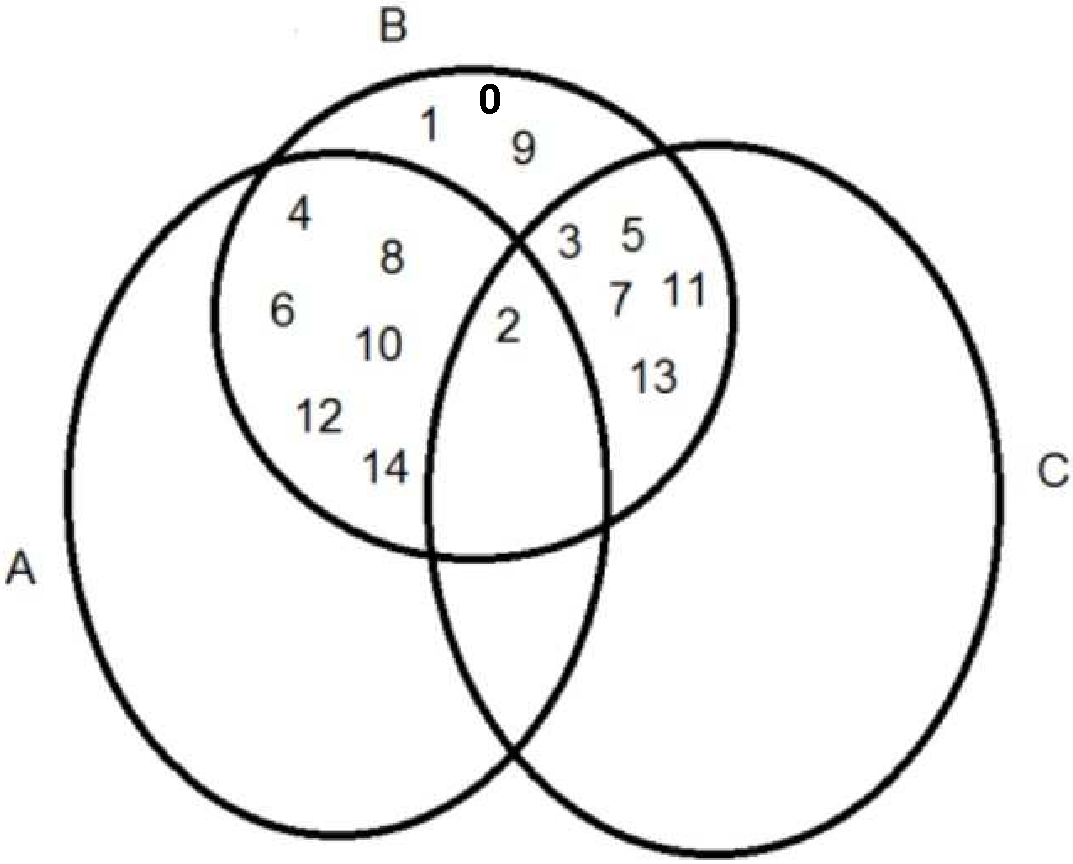
\includegraphics[width=.4\linewidth]{Figs/conjuntos-cropped.pdf}
    \end{center}

\end{Gabarito}
\begin{Gabarito}{18}
~

    \begin{center}
        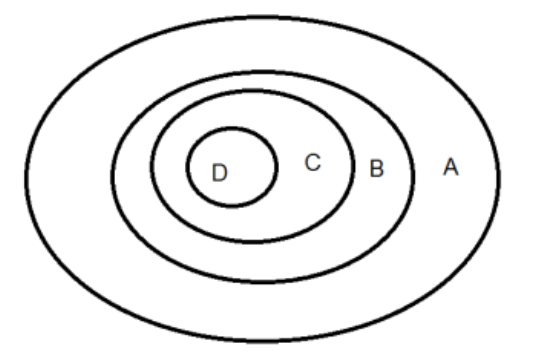
\includegraphics[width=.4\linewidth]{Figs/conjuntos2.png}
    \end{center}
\end{Gabarito}
\begin{Gabarito}{19}
~

    \begin{multicols}{2}
    \begin{enumerate}[a)]
        \item $\{1,2,3,4,5\}$
        \item $\{1,3\}$
        \item $\{5,7,9,11,...\}$
        \item $\{0,5,6,7,8,9,11,13,15,17,...\}$
        \item $\{ 4, 2, \infty\}$
    \end{enumerate}
\end{multicols}

\end{Gabarito}
\begin{Gabarito}{20}
~

    \begin{enumerate}[a)]
        \item $\{(a,x),(a,y),(b,x),(b,y),(c,x),(c,y)\}$
        \item $\{(0,a),(0,b),(0,c),(1,a),(1,b),(1,c)\}$
    \end{enumerate}
\end{Gabarito}
\begin{Gabarito}{21}
~

    \begin{enumerate}[a)]
    \item
    \begin{multicols}{2}
        \begin{itemize}
            \item $A \cup (B \cap \overline{B})$
            \item $A \cup \emptyset$
            \item $A$
        \end{itemize}

        \begin{itemize}
            \item (distributividade)
            \item (complemento)
            \item (elemento neutro)
        \end{itemize}
    \end{multicols}

    \item

    Correção: $A \cap (B \cup \overline{A}) = B \cap A$

    \begin{multicols}{2}
        \begin{itemize}
            \item $(A \cap B) \cup (A \cap \overline{A})$
            \item $(A \cap B) \cup \emptyset$
            \item $(A \cap B)$
            \item $(B \cap A)$
        \end{itemize}

        \begin{itemize}
            \item (distributividade)
            \item (complemento)
            \item (elemento neutro)
            \item (comutatividade)
        \end{itemize}
    \end{multicols}
\end{enumerate}
\end{Gabarito}
\begin{Gabarito}{22}
~

    $A=\{1,3,5,6,7,8,9\}$ e $B=\{2,3,6,9,10\}$
\end{Gabarito}
\begin{Gabarito}{23}
~

    $X=\{1,3,5\}$
\end{Gabarito}
\begin{Gabarito}{24}
~


    a
\end{Gabarito}
 %imprime as soluções
\end{document}
